\documentclass[11pt,class=report,crop=false]{standalone}
\usepackage{exo7hilisit}

\begin{document}


\entete{Hilisit}{Capacité mathématiques}

\titre{\'Equations différentielles -- Partie 1 : Primitives}

\bigskip
\bigskip


%%%%%%%%%%%%%%%%%%%%%%%%%%%%%%%%%%%%%%%%%%%%%%%%%%%%%%%%%%%%
%\section{Primitive}

\exercice{}
\enonce
Mettre en correspondance chaque fonction $f$ avec une de ses primitives $F$. 
 \begin{itemize}
  \item $f_1(x) = -6\sin(2x)$, $f_2(x) = 2x$, $f_3(x) = (x+1)e^x$, $f_4(x) = -6\sin(3x)$, $f_5(x) = 2xe^{x^2}$, $f_6(x)=2x+2$.
  \item $F_a(x) = 2\cos(3x)$, $F_b(x) = 3\cos(2x)$, $F_c(x) = (x+1)^2$, $F_d(x) = x^2+1$, $F_e(x) = e^{x^2}$, $F_f(x) = xe^x$. 
\end{itemize} 
\finenonce

\indication
$F$ est une primitive de $f$ si $F'(x)=f(x)$ (pour tout $x$ de l'ensemble de définition).
\finindication

\correction
\sauteligne
\begin{enumerate}
  \item $F_a(x) = 2\cos(3x)$, $F_a'(x) = f_4(x) = -6\sin(3x)$.
  \item $F_b(x) = 3\cos(2x)$, $F_b'(x) = f_1(x) = -6\sin(2x)$.
  \item $F_c(x) = (x+1)^2$, $F_c'(x) = f_6(x) = 2x+2$.
  \item $F_d(x) = x^2+1$, $F_d'(x) = f_2(x) = 2x$.
  \item $F_e(x) = e^{x^2}$, $F_e'(x) = f_5(x) = 2xe^{x^2}$.
  \item $F_f(x) = xe^x$, $F_f'(x) = f_3(x) = (x+1)e^x$.
\end{enumerate}
\fincorrection
\finexercice


\exercice{}
\enonce
Pour chacune des fonctions $f$ suivantes, déterminer une primitive $F$.
\begin{enumerate}
  \item $f_1(x) = -\cos(2x)$
  \item $f_2(x) = x^3-7x^2+1$
  \item $f_3(x) = \frac{1}{2x-1}$ (sur $]-\frac12,+\infty[$)
  \item $f_4(x) = e^{\pi x-3}$
  \item $f_5(x) = -(x-2)^2$
  \item $f_6(x) = \sin(8(x+1))$
\end{enumerate} 
\finenonce

\indication
Il s'agit de trouver une fonction $F$ telle que $F'(x) = f(x)$. Il faut bien connaître ses formules des dérivées usuelles.
\finindication

\correction
\sauteligne
\begin{enumerate}
  \item $F_1(x) = -\frac12\sin(2x)$, on vérifie que $F_1'(x) = f_1(x)$.
  \item $F_2(x) = \frac14x^4-\frac73x^3+x$, car une primitive de $x^k$ est $\frac{1}{k+1}x^{x+1}$ (pour $k \ne -1$).
  \item $F_3(x) = \frac12\ln(2x-1)$ car $(\ln(u))' = \frac{u'}{u}$ avec ici $u(x)=2x-1$.
  \item $F_4(x) = \frac{1}{\pi}e^{\pi x-3}$ car $(e^u)' = u'e^u$ avec ici $u(x)=\pi x-3$.
  \item $F_5(x) = -\frac{x^3}{3}+2x^2-4x$ car $f_5(x) = -x^2+4x-4$. On peut aussi écrire $F_5(x) = -\frac13(x-2)^3$. 
  \item $F_6(x) = -\frac18\cos(8(x+1))$ car $(\cos(u))' = -u' \sin(u)$.
\end{enumerate}
Dans tous les cas, si $F$ est une primitive, alors pour toute constante $C$, $F+C$ est aussi une primitive.
\fincorrection
\finexercice


\exercice{}
\enonce
\sauteligne
\begin{enumerate}
  \item 
  \begin{enumerate}
    \item Quelle est la dérivée de la fonction $x \mapsto u^k(x)$ où $x \mapsto u(x)$ est une fonction et $k$ un entier ?
    \item Calculer les dérivées des fonctions définies par $(x^4+7x^3+2)^3$, $\cos^3(2x)$, $\ln^2(x)$, $\frac{1}{(x^2+1)^2}$.
    \item Déterminer une primitive des fonctions définies par $x(x^2+5)^5$, $\sin(x) \cos^3(x)$, $\frac{\ln^n(x)}{x}$ (où $n\ge0$).
  \end{enumerate} 

  \item 
  \begin{enumerate}
    \item Quelle est la dérivée de la fonction $x \mapsto e^{u(x)}$ où $x \mapsto u(x)$ est une fonction ?
    \item Calculer les dérivées des fonctions définies par $e^{-5x}$, $e^{x^3-2x}$, $e^{\sin(3x)}$, $e^{1/x}$.
    \item Déterminer une primitive des fonctions définies par $e^{8x+1}$, $xe^{x^2+1}$, $\frac{e^{\sqrt x}}{\sqrt x}$.
  \end{enumerate} 


  \item 
  \begin{enumerate}
    \item Quelle est la dérivée de la fonction $x \mapsto \ln(u(x))$ où $x \mapsto u(x)$ est une fonction strictement positive ?
    \item Calculer les dérivées des fonctions définies par $\ln(x^3-2)$, $\ln(e^x+e^{-x})$, $\ln(1/x)$, $\ln(\cos(x^2))$.
    \item Déterminer une primitive des fonctions définies par $\frac{1}{x+4}$ (sur $]-4,+\infty[$), $\frac{x}{x^2+4}$ (sur $\Rr$), $\frac{\cos(x)}{\sin(x)}$ (pour les $x$ où $\sin(x)>0$).
  \end{enumerate} 

\end{enumerate} 
\finenonce

\indication
La dérivée d'une composition $f(u(x))$ est $u'(x) f'(u(x))$.
Pour déterminer les primitives il faut reconnaître la fonction sous une forme $u'(x) f'(u(x))$, afin de déterminer qu'une primitive est $f(u(x))$.
\finindication

\correction
\sauteligne
\begin{enumerate}
  \item 
  \begin{enumerate}
    \item La dérivée de $u^k(x)$ est $ku'(x)u^{k-1}(x)$.
    \item 
    \begin{itemize}
      \item La dérivée de $(x^4+7x^3+2)^3$ est $3(4x^3+21x^2)(x^4+7x^3+2)^2$.
      \item La dérivée de $\cos^3(2x)$ est $-6\sin(2x)\cos^2(2x)$.
      \item La dérivée de $\ln^2(x)$ est $\frac2x\ln(x)$. 
      \item La dérivée de $\frac{1}{(x^2+1)^2} = (x^2+1)^{-2}$ est $-2(2x)(x^2+1)^{-3}=\frac{-4x}{(x^2+1)^3}$.
    \end{itemize} 
    \item 
    \begin{itemize}
      \item Une primitive de $x(x^2+5)^5 = \frac1{12} \cdot 6 \cdot (2x) \cdot (x^2+5)^5$ est $\frac1{12} (x^2+5)^6$.
      \item Une primitive de $\sin(x) \cos^3(x)$ est $-\frac14\cos^4(x)$.
      \item Une primitive de $\frac{\ln^n(x)}{x}$ est $\frac{1}{n+1}\ln^{n+1}(x)$.
    \end{itemize} 
  \end{enumerate} 

  \item 
  \begin{enumerate}
    \item La dérivée de $e^{u(x)}$ est $u'(x)e^{u(x)}$.
    \item 
    \begin{itemize}
      \item La dérivée de $e^{-5x}$ est $-5e^{-5x}$.
      \item La dérivée de $e^{x^3-2x}$ est $(3x^2-2)e^{x^3-2x}$.
      \item La dérivée de $e^{\sin(3x)}$ est $3\cos(3x)e^{\sin(3x)}$.
      \item La dérivée de $e^{1/x}$ est $-\frac1{x^2}e^{1/x}$.
    \end{itemize} 

    \item 
    \begin{itemize}
      \item Une primitive de $e^{8x+1}$ est $\frac18e^{8x+1}$.
      \item Une primitive de $xe^{x^2+1}$ est $\frac12e^{x^2+1}$ 
      \item Une primitive de $\frac{e^{\sqrt x}}{\sqrt x}$ est $2e^{\sqrt x}$.
    \end{itemize} 
  \end{enumerate} 


  \item 
  \begin{enumerate}
    \item La dérivée de $\ln(u(x))$ est $\frac{u'(x)}{u(x)}$.
    \item 
    \begin{itemize}
      \item La dérivée de $\ln(x^3-2)$ est $\frac{3x^2}{x^3-2}$.
      \item La dérivée de $\ln(e^x+e^{-x})$ est $\frac{e^x-e^{-x}}{e^x+e^{-x}}$.
      \item La dérivée de $\ln(1/x)$ est $-\frac{1}{x}$ (c'est plus facile si on a remarqué que $\ln(1/x)=-\ln(x)$ !).
      \item La dérivée de $\ln(\cos(x^2))$ est $\frac{-2x\sin(x^2)}{\cos(x^2)}$.
    \end{itemize}

    \item 
    \begin{itemize}
      \item Une primitive de $\frac{1}{x+4}$ est $\ln(x+4)$.
      \item Une primitive de $\frac{x}{x^2+4}$ est $\frac12\ln(x^2+4)$.
      \item Une primitive de $\frac{\cos(x)}{\sin(x)}$ est $\ln(\sin(x))$.
    \end{itemize} 
  \end{enumerate} 

\end{enumerate} 
\fincorrection
\finexercice


\exercice{}
\enonce
\sauteligne
 \begin{enumerate}
  \item Pour la fonction $f$ représentée ci-dessous, déterminer quel est le graphe de la fonction $F_i$ qui correspond à une primitive de $f$.
\begin{center}
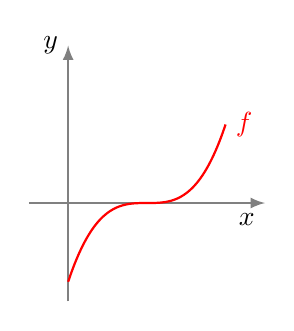
\begin{tikzpicture}[scale=1]
  \draw[->,>=latex,thick,gray] (-0.5,0) -- (2.5,0) node[below left,black] {$x$};
  \draw[->,>=latex,thick,gray] (0,-1.25) -- (0,2) node[left,black] {$y$};
  \draw[thick, color=red,domain=0:2, smooth,samples=50] plot (\x,{(\x-1)^3}) node[right]{$f$};
\end{tikzpicture}
\end{center}

\begin{center}
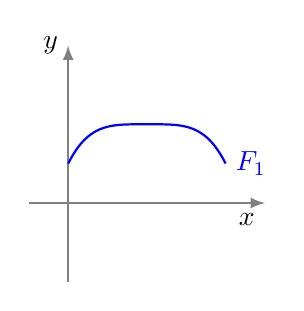
\begin{tikzpicture}[scale=1]
  \draw[->,>=latex,thick,gray] (-0.5,0) -- (2.5,0) node[below left,black] {$x$};
  \draw[->,>=latex,thick,gray] (0,-1) -- (0,2) node[left,black] {$y$};
  \draw[thick, color=blue,domain=0:2, smooth,samples=50] plot (\x,{-1/2*(\x-1)^4+1}) node[right]{$F_1$};
\end{tikzpicture}
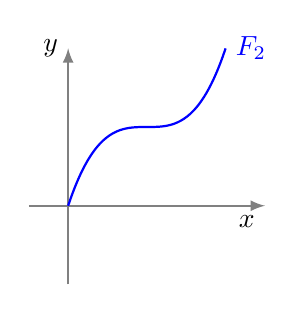
\begin{tikzpicture}[scale=1]
  \draw[->,>=latex,thick,gray] (-0.5,0) -- (2.5,0) node[below left,black] {$x$};
  \draw[->,>=latex,thick,gray] (0,-1) -- (0,2) node[left,black] {$y$};
  \draw[thick, color=blue,domain=0:2, smooth,samples=50] plot (\x,{(\x-1)^3+1}) node[right]{$F_2$};
\end{tikzpicture}
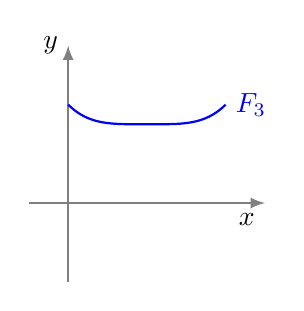
\begin{tikzpicture}[scale=1]
  \draw[->,>=latex,thick,gray] (-0.5,0) -- (2.5,0) node[below left,black] {$x$};
  \draw[->,>=latex,thick,gray] (0,-1) -- (0,2) node[left,black] {$y$};
  \draw[thick, color=blue,domain=0:2, smooth,samples=50] plot (\x,{1/4*(\x-1)^4+1}) node[right]{$F_3$};
\end{tikzpicture}
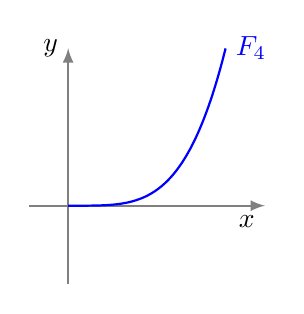
\begin{tikzpicture}[scale=1]
  \draw[->,>=latex,thick,gray] (-0.5,0) -- (2.5,0) node[below left,black] {$x$};
  \draw[->,>=latex,thick,gray] (0,-1) -- (0,2) node[left,black] {$y$};
  \draw[thick, color=blue,domain=0:2, smooth,samples=50] plot (\x,{1/8*\x^4}) node[right]{$F_4$};
\end{tikzpicture}
\end{center}

  \item Pour la fonction $f$ représentée ci-dessous, déterminer quel est le graphe de la fonction $F_i$ qui correspond à une primitive de $f$.
\begin{center}
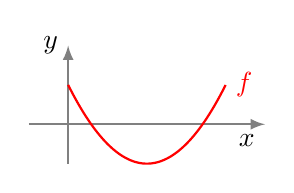
\begin{tikzpicture}[scale=1]
  \draw[->,>=latex,thick,gray] (-0.5,0) -- (2.5,0) node[below left,black] {$x$};
  \draw[->,>=latex,thick,gray] (0,-0.5) -- (0,1) node[left,black] {$y$};
  \draw[thick, color=red,domain=0:2, smooth,samples=50] plot (\x,{(\x-1)^2-1/2}) node[right]{$f$};
\end{tikzpicture}
\end{center}

\begin{center}
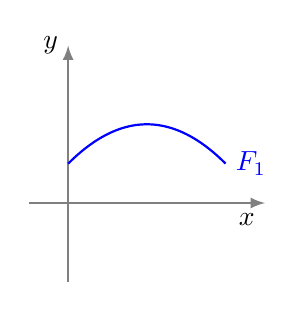
\begin{tikzpicture}[scale=1]
  \draw[->,>=latex,thick,gray] (-0.5,0) -- (2.5,0) node[below left,black] {$x$};
  \draw[->,>=latex,thick,gray] (0,-1) -- (0,2) node[left,black] {$y$};
  \draw[thick, color=blue,domain=0:2, smooth,samples=50] plot (\x,{-1/2*(\x-1)^2+1}) node[right]{$F_1$};
\end{tikzpicture}
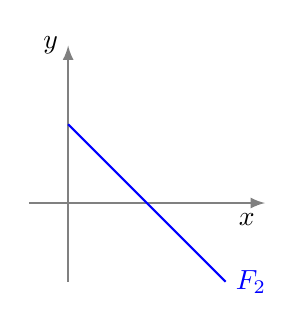
\begin{tikzpicture}[scale=1]
  \draw[->,>=latex,thick,gray] (-0.5,0) -- (2.5,0) node[below left,black] {$x$};
  \draw[->,>=latex,thick,gray] (0,-1) -- (0,2) node[left,black] {$y$};
  \draw[thick, color=blue,domain=0:2, smooth,samples=50] plot (\x,{-\x+1}) node[right]{$F_2$};
\end{tikzpicture}
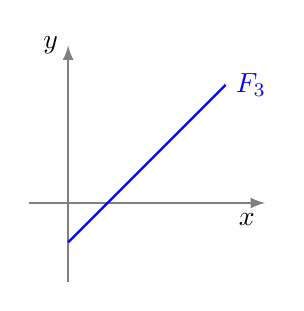
\begin{tikzpicture}[scale=1]
  \draw[->,>=latex,thick,gray] (-0.5,0) -- (2.5,0) node[below left,black] {$x$};
  \draw[->,>=latex,thick,gray] (0,-1) -- (0,2) node[left,black] {$y$};
  \draw[thick, color=blue,domain=0:2, smooth,samples=50] plot (\x,{\x-0.5}) node[right]{$F_3$};
\end{tikzpicture}
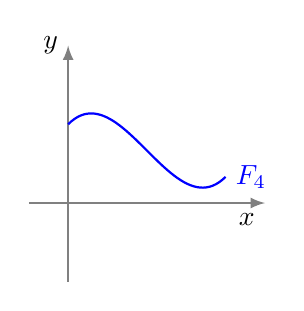
\begin{tikzpicture}[scale=1]
  \draw[->,>=latex,thick,gray] (-0.5,0) -- (2.5,0) node[below left,black] {$x$};
  \draw[->,>=latex,thick,gray] (0,-1) -- (0,2) node[left,black] {$y$};
  \draw[thick, color=blue,domain=0:2, smooth,samples=50] plot (\x,{2*(\x/2 - \x^2 + \x^3/3)+1}) node[right]{$F_4$};
\end{tikzpicture}
\end{center}

\end{enumerate} 
\finenonce

\indication
Il faut utiliser que la dérivée de $F$ est $f$ et utiliser le signe (et non pas la monotonie) de $f$ pour déterminer là où $F$ est croissante ou décroissante.
\finindication

\correction 
\sauteligne

Comme la dérivée de $F$ est $f$, là où $f$ est positive, $F$ est croissante ; là où $f$ est négative, $F$ est décroissante.
\begin{enumerate}
  \item $f = F'$ est négative puis positive : $F$ doit être d'abord décroissante, puis ensuite croissante. Ainsi il s'agit de $F_3$.
  \item $f = F'$ est positive, négative puis à nouveau positive. Donc $F$ est croissante, décroissante puis à nouveau croissante. Il s'agit de $F_4$.
\end{enumerate} 
\fincorrection
\finexercice


\end{document}
